\documentclass[conference]{IEEEtran}
\IEEEoverridecommandlockouts
% The preceding line is only needed to identify funding in the first footnote. If that is unneeded, please comment it out.
\usepackage{cite}
\usepackage{amsmath,amssymb,amsfonts}
\usepackage{algorithmic}
\usepackage{graphicx}
\usepackage{textcomp}
\usepackage{xcolor}
\def\BibTeX{{\rm B\kern-.05em{\sc i\kern-.025em b}\kern-.08em
    T\kern-.1667em\lower.7ex\hbox{E}\kern-.125emX}}
\begin{document}

\title{Blood pressure and Body temperature IOT\\
}

\author{\IEEEauthorblockN{1\textsuperscript{st} MD.Eyamin Molla}
ID:19202103209 \\
Intake:44 , Section:06\\
\IEEEauthorblockA{\textit{Dept. of CSE.} \\
\textit{(BUBT)}\\
19202103209@cse.bubt.edu.bd}
\and
\IEEEauthorblockN{2\textsuperscript{nd} MD. Rakibul Rahman Zihad}
ID:19201103082 \\
Intake:44 , Section:06\\
\IEEEauthorblockA{\textit{Dept. of CSE.} \\
\textit{(BUBT)}\\
19201103082@cse.bubt.edu.bd}
\and
\IEEEauthorblockN{3\textsuperscript{rd} MD.Mehedi Hasan}
ID:19202103474 \\
Intake:44 , Section:06\\
\IEEEauthorblockA{\textit{Dept. of CSE.} \\
\textit{(BUBT)}\\
19202103474@cse.bubt.edu.bd}
\and
\IEEEauthorblockN{4\textsuperscript{th} MD. Nahian Islam}
ID:19201103028 \\
Intake:44 , Section:06\\
\IEEEauthorblockA{\textit{Dept. of CSE.} \\
\textit{(BUBT)}\\
19201103028@cse.bubt.edu.bd}
\and
\IEEEauthorblockN{5\textsuperscript{th} MD. Mohibbullah}
ID:19201103101 \\
Intake:44 , Section:06\\
\IEEEauthorblockA{\textit{Dept. of CSE.} \\
\textit{(BUBT)}\\
19201103101@cse.bubt.edu.bd}

}
\maketitle


\section{Introduction}
The Internet of Things (IoT) has revolutionized the way we interact with the world around us. One of the most promising applications of IoT is in the healthcare industry, where it can be used to monitor patient health remotely and in real-time. In this project, we aim to develop an IoT-based health monitoring system that can measure the blood pressure and temperature of a patient and transmit the data to a remote server for analysis.The system consists of a wearable device that is worn by the patient, which is capable of measuring their blood pressure and temperature. The device is equipped with sensors that can detect the patient's vital signs and transmit the data to a central server using wireless communication. The server is responsible for analyzing the data and providing feedback to the patient and their healthcare provider.The main goal of this project is to provide a non-invasive and easy-to-use method for monitoring patient health remotely. By using IoT technology, we can provide patients with a convenient way to track their vital signs and receive feedback on their health status in real-time. The system can also be used by healthcare providers to monitor the health of their patients remotely, allowing them to provide timely interventions when necessary.
High blood pressure and fever are common health issues that can have serious consequences if not identified and treated promptly. However, monitoring these conditions can be challenging, especially for individuals who have busy schedules and may not have access to medical facilities. In addition, traditional methods of monitoring blood pressure and body temperature require manual recording and tracking, which can be time-consuming and prone to errors.
The proposed project aims to address these challenges by developing a system that can monitor and display blood pressure and body temperature readings in real time. The system will provide individuals with an easy and efficient way to monitor their health and identify any potential health issues. The use of a 16x2 crystal display will enable individuals to view their readings in real-time, while the integration of sensors and a micro-controller will provide accurate and reliable readings. The use of a thingspeak  will allow individuals to store and analyze their data, enabling them to track trends and patterns in their readings over time.Overall, this project has the potential to revolutionize the way we approach healthcare, by providing a more convenient and efficient way to monitor patient health. With the continued growth of IoT technology, we expect to see more applications of this technology in the healthcare industry in the future.

\section{Literature Review}
    The Internet of Things (IoT) has revolutionized healthcare by providing efficient and effective remote patient monitoring. One of the critical health parameters that require continuous monitoring is blood pressure and temperature. This project aims to design an IoT-based health monitoring system that can monitor the blood pressure and temperature of patients remotely. Various studies have been conducted on IoT-based health monitoring systems for blood pressure and temperature. \\
    \begin{itemize}

  \item {In a study by S. M. Riazul Islam et al. (2015), an IoT-based health monitoring system was designed that could monitor blood pressure, heart rate, and body temperature remotely. The system consisted of a wearable device and a mobile application that could be used to monitor and store the patient's data.}
\item {Another study by Y. Liu et al. (2016) proposed an IoT-based blood pressure monitoring system that used a wearable device to measure the blood pressure and a mobile application to display the results. The system was also capable of sending alerts to healthcare providers in case of abnormal blood pressure readings.}

\item {In a study by M. Ali et al. (2018), an IoT-based temperature monitoring system was designed that used a wireless sensor network to measure the temperature of patients remotely. The system could also send alerts to healthcare providers in case of abnormal temperature readings.}

\item {In another study by S. Sharma et al. (2020), an IoT-based blood pressure monitoring system was designed that used a smartwatch to measure the blood pressure and a mobile application to display the results. The system also had a feature that could track the patient's location and send alerts to emergency services in case of a medical emergency.}\\
The literature review shows that IoT-based health monitoring systems for blood pressure and temperature are being extensively researched. These systems can provide efficient and effective remote patient monitoring, which can improve patient outcomes and reduce healthcare costs. The proposed IoT-based health monitoring system for blood pressure and temperature can be a useful tool for healthcare providers to monitor their patients remotely.
    




\end{itemize}
    \section{Proposed Systems}
    The Internet of Things (IoT) is rapidly becoming an integral part of our lives, with the ability to connect a vast number of devices to the internet. IoT has enabled us to gather data from numerous sources, which can be used to improve our lives in many ways. One of the areas where IoT has the potential to make a significant impact is healthcare. In this project report, we propose an IoT health monitoring system that can measure blood pressure and temperature.
The proposed system is an IoT health monitoring system that can measure blood pressure and temperature. The system consists of two parts: a hardware component and a software component.
The hardware component consists of a blood pressure sensor, a temperature sensor, a micro-controller, and a Wi-Fi module. The blood pressure sensor measures the user's blood pressure, while the temperature sensor measures the user's body temperature. The micro-controller collects the data from the sensors and sends it to the Wi-Fi module, which transmits the data to the cloud server.
The software component consists of a cloud server, a database, and a user interface. The cloud server receives the data transmitted by the Wi-Fi module and stores it in the database. The user interface allows the user to view their blood pressure and temperature readings, as well as any trends over time.
The proposed IoT health monitoring system has several benefits. Firstly, it allows individuals to monitor their blood pressure and temperature from the comfort of their own home, without having to visit a doctor. This can be particularly useful for individuals with chronic conditions that require regular monitoring. Secondly, the system can provide doctors with real-time data, allowing them to make more informed decisions about a patient's health. Finally, the system can help identify trends over time, allowing individuals and doctors to detect any changes in the user's health.
Overall, the proposed IoT health monitoring system has the potential to revolutionize healthcare by providing individuals with a convenient way to monitor their health and by providing doctors with real-time data. With the increasing prevalence of IoT devices, we believe that this system has the potential to become an essential tool in healthcare.\\
\newline
\textbf{Hardware Requirements}\\
\textbullet Arduino Uno\\
\textbullet ESP8266 Wifi Moudle\\
\textbullet Blood pressure sensor\\
\textbullet Temperature sensor\\
\textbullet Buzzer \\
\textbullet LED light\\
\textbullet 16*2 lcd display\\
\textbullet Breadboard\\
\textbullet Jumper wires\\

\textbf{Software Requirements:}\\
\textbullet Arduino IDE\\
\textbullet MQTT protocol\\
\textbullet Cloud-based platform for data storage and visualization\\
\textbf{Hardware Setup}\\
The first step is to connect the hardware components. Connect the blood pressure sensor and temperature sensor to the Arduino Uno using jumper wires. Connect the Wi-Fi module to the Arduino.

    \section{Methodology}
The IoT health monitoring system project aims to design and develop a device that can monitor the blood pressure and body temperature of a patient remotely. The methodology used in this project involves a systematic approach that includes several stages such as research, design, implementation, and testing. In the research stage, the team conducted a thorough literature review to identify the latest technologies and trends in the field of IoT health monitoring systems. This stage also involved identifying the different components required for the device, such as sensors, microcontrollers, communication modules, and power sources. The team also selected the appropriate components based on the research conducted earlier.In the implementation stage, the team assembled the device and tested it to ensure that it met the desired specifications. This stage involved programming the microcontroller, configuring the communication module, and testing the sensors.\\
\begin{figure}[h]
    \centering
    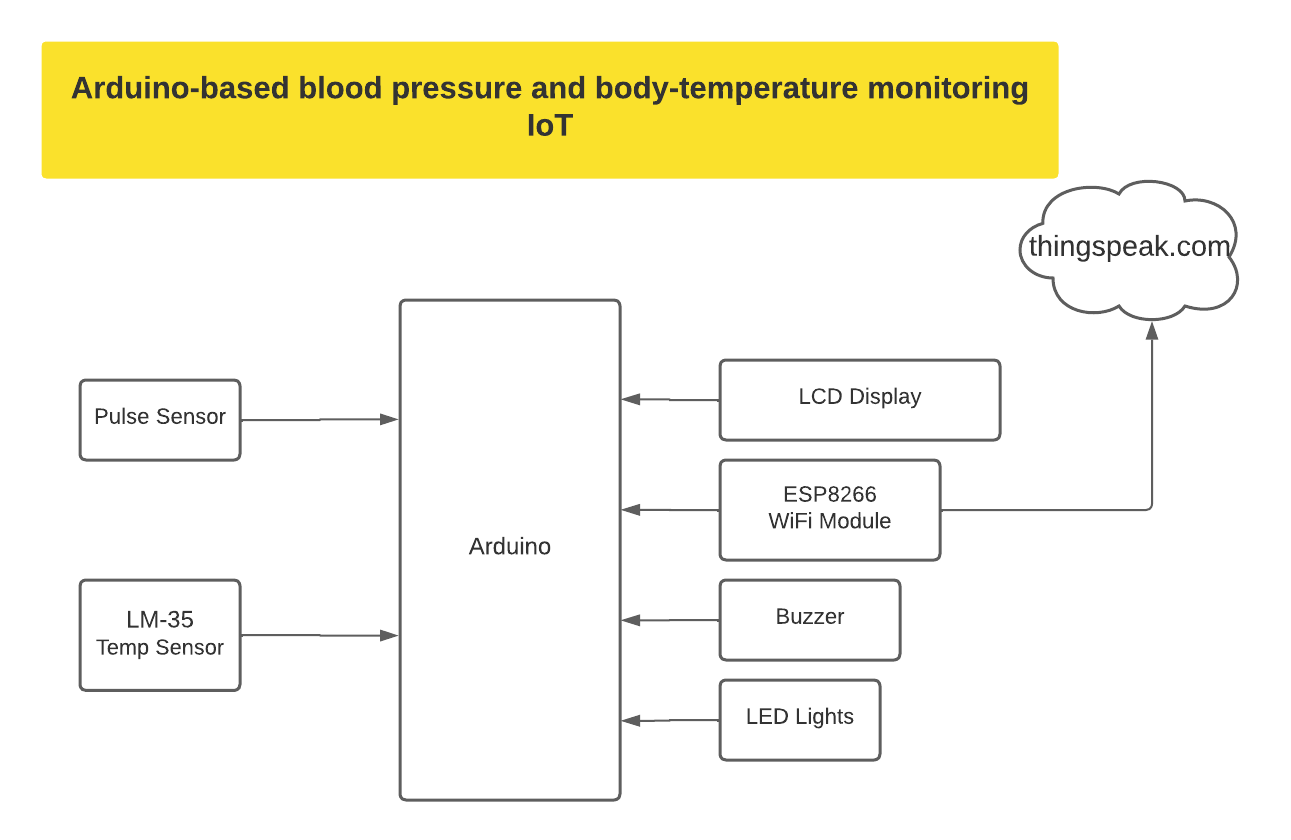
\includegraphics[width=.5\textwidth]{fullfig.png}
    \caption{Proposed Diagram}
    \label{fig:mesh1}
\end{figure}
The first step in the project is to understand the requirements of the IoT Health Monitoring System for Blood Pressure and Temperature. This includes identifying the stakeholders and their needs, defining the functional and non-functional requirements, and determining the system's scope.
Requirement Analysis for IoT Health Monitoring System for Blood Pressure and Temperature:
Following are functional requirements of IoT-based health monitoring system for blood pressure and temperature:
The system should be able to measure patients' blood pressure accurately and in real time. Capable of measuring patients body temperature accurately and in real time. Data is transmitted to a remote server or a mobile application.
Also, the system should be able to generate reports on daily, weekly and monthly basis. So the system is easy to use and manage.
Following are the non-functional requirements of IoT-based health monitoring system for blood pressure and temperature:
The system is reliable and accurate. The system is used securely to prevent unauthorized access to patient data. Used to accommodate a large number of patients.The system is cost-effective, and made user-friendly.In this phase, the overall architecture of the IoT Health Monitoring System is designed. This includes the hardware and software components, the communication protocols, and the data storage and processing mechanisms.
The hardware implementation involves selecting and integrating the necessary sensors and other components required to measure and monitor the blood pressure and temperature. This includes selecting the appropriate micro controller, connecting the sensors to the micro controller, and implementing the necessary circuits.
The software implementation involves writing the code for the micro controller to read the sensor data and transmit it to the cloud platform. This also includes developing the mobile and web applications to visualize and analyze the data received from the sensors.
The IoT Health Monitoring System is tested for functionality, reliability, and security. The system is then deployed in the field, and its performance is monitored.
The IoT Health Monitoring System requires ongoing maintenance and support to ensure its continued operation. This includes monitoring the system's performance, updating the software, and providing customer support.Overall, the IoT Health Monitoring System for Blood Pressure and Temperature is a complex system that requires a comprehensive methodology to ensure its successful implementation. The methodology described above provides a systematic approach to design, implement, and deploy the IoT Health Monitoring System while ensuring its reliability, security, and performance.
\section{Implementation and result analysis}
IoT based health monitoring system can play an important role in monitoring vital health parameters such as blood pressure and temperature in real-time. This project aims to develop an IoT based health monitoring system that can monitor blood pressure and temperature and send the data to a cloud-based platform for further analysis and visualization.\\
\begin{figure}[h]
    \centering
    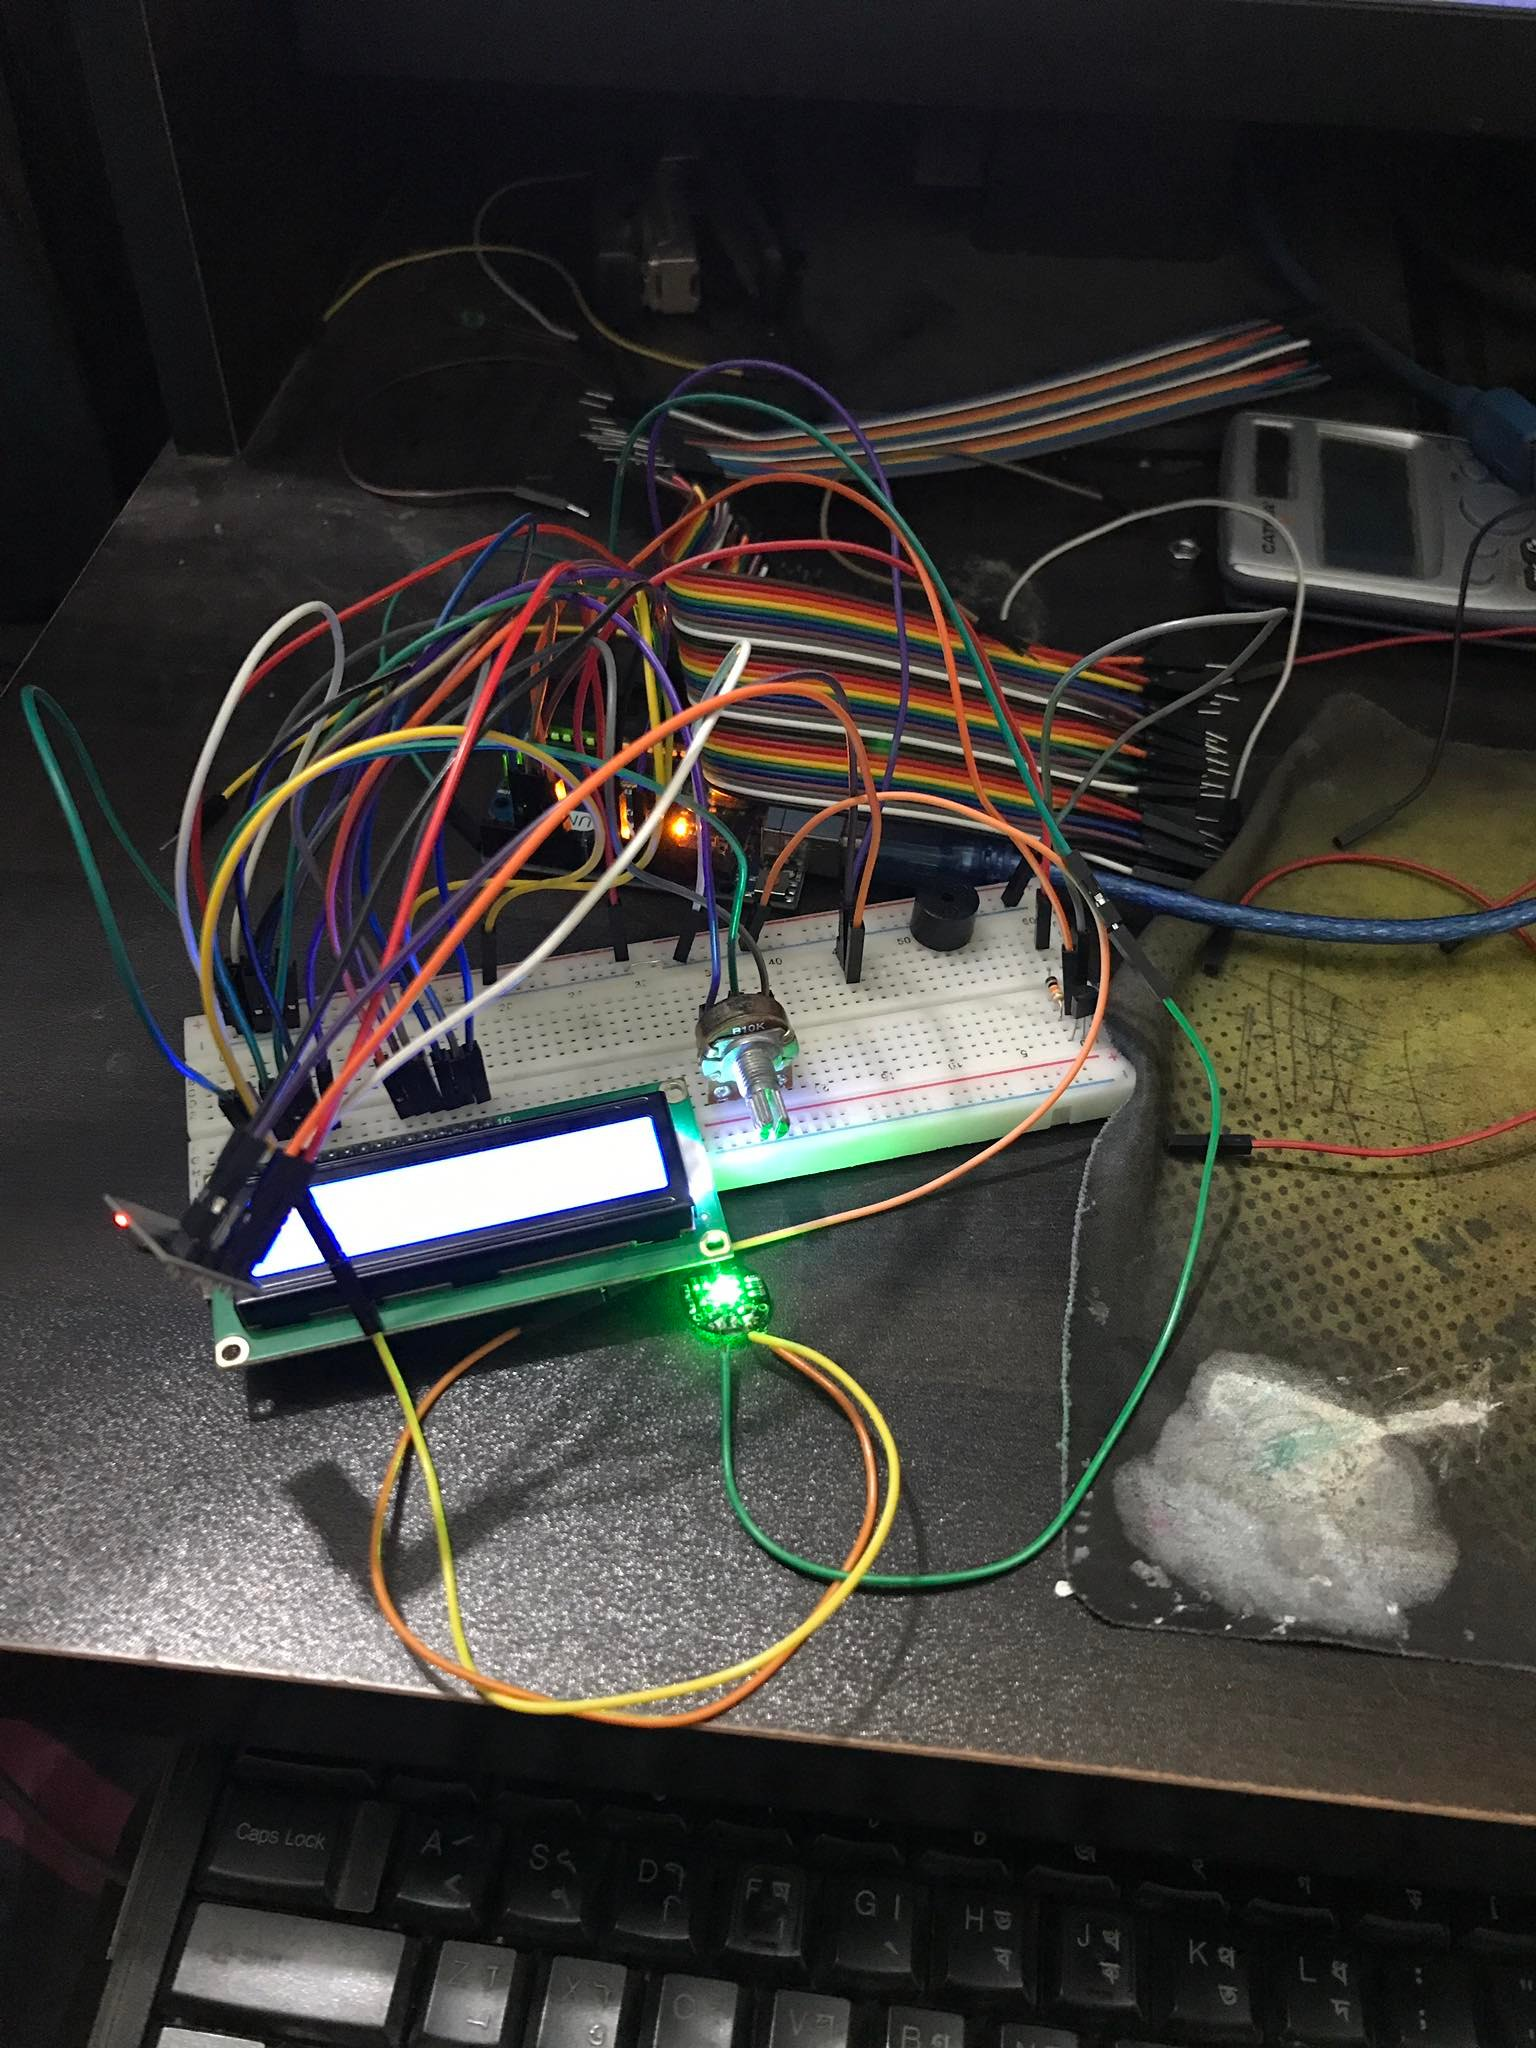
\includegraphics[width=0.25\textwidth]{project_pic.jpg}
    \caption{Project Image}
    \label{fig:mesh1}
\end{figure}
\begin{figure}[h]
    \centering
    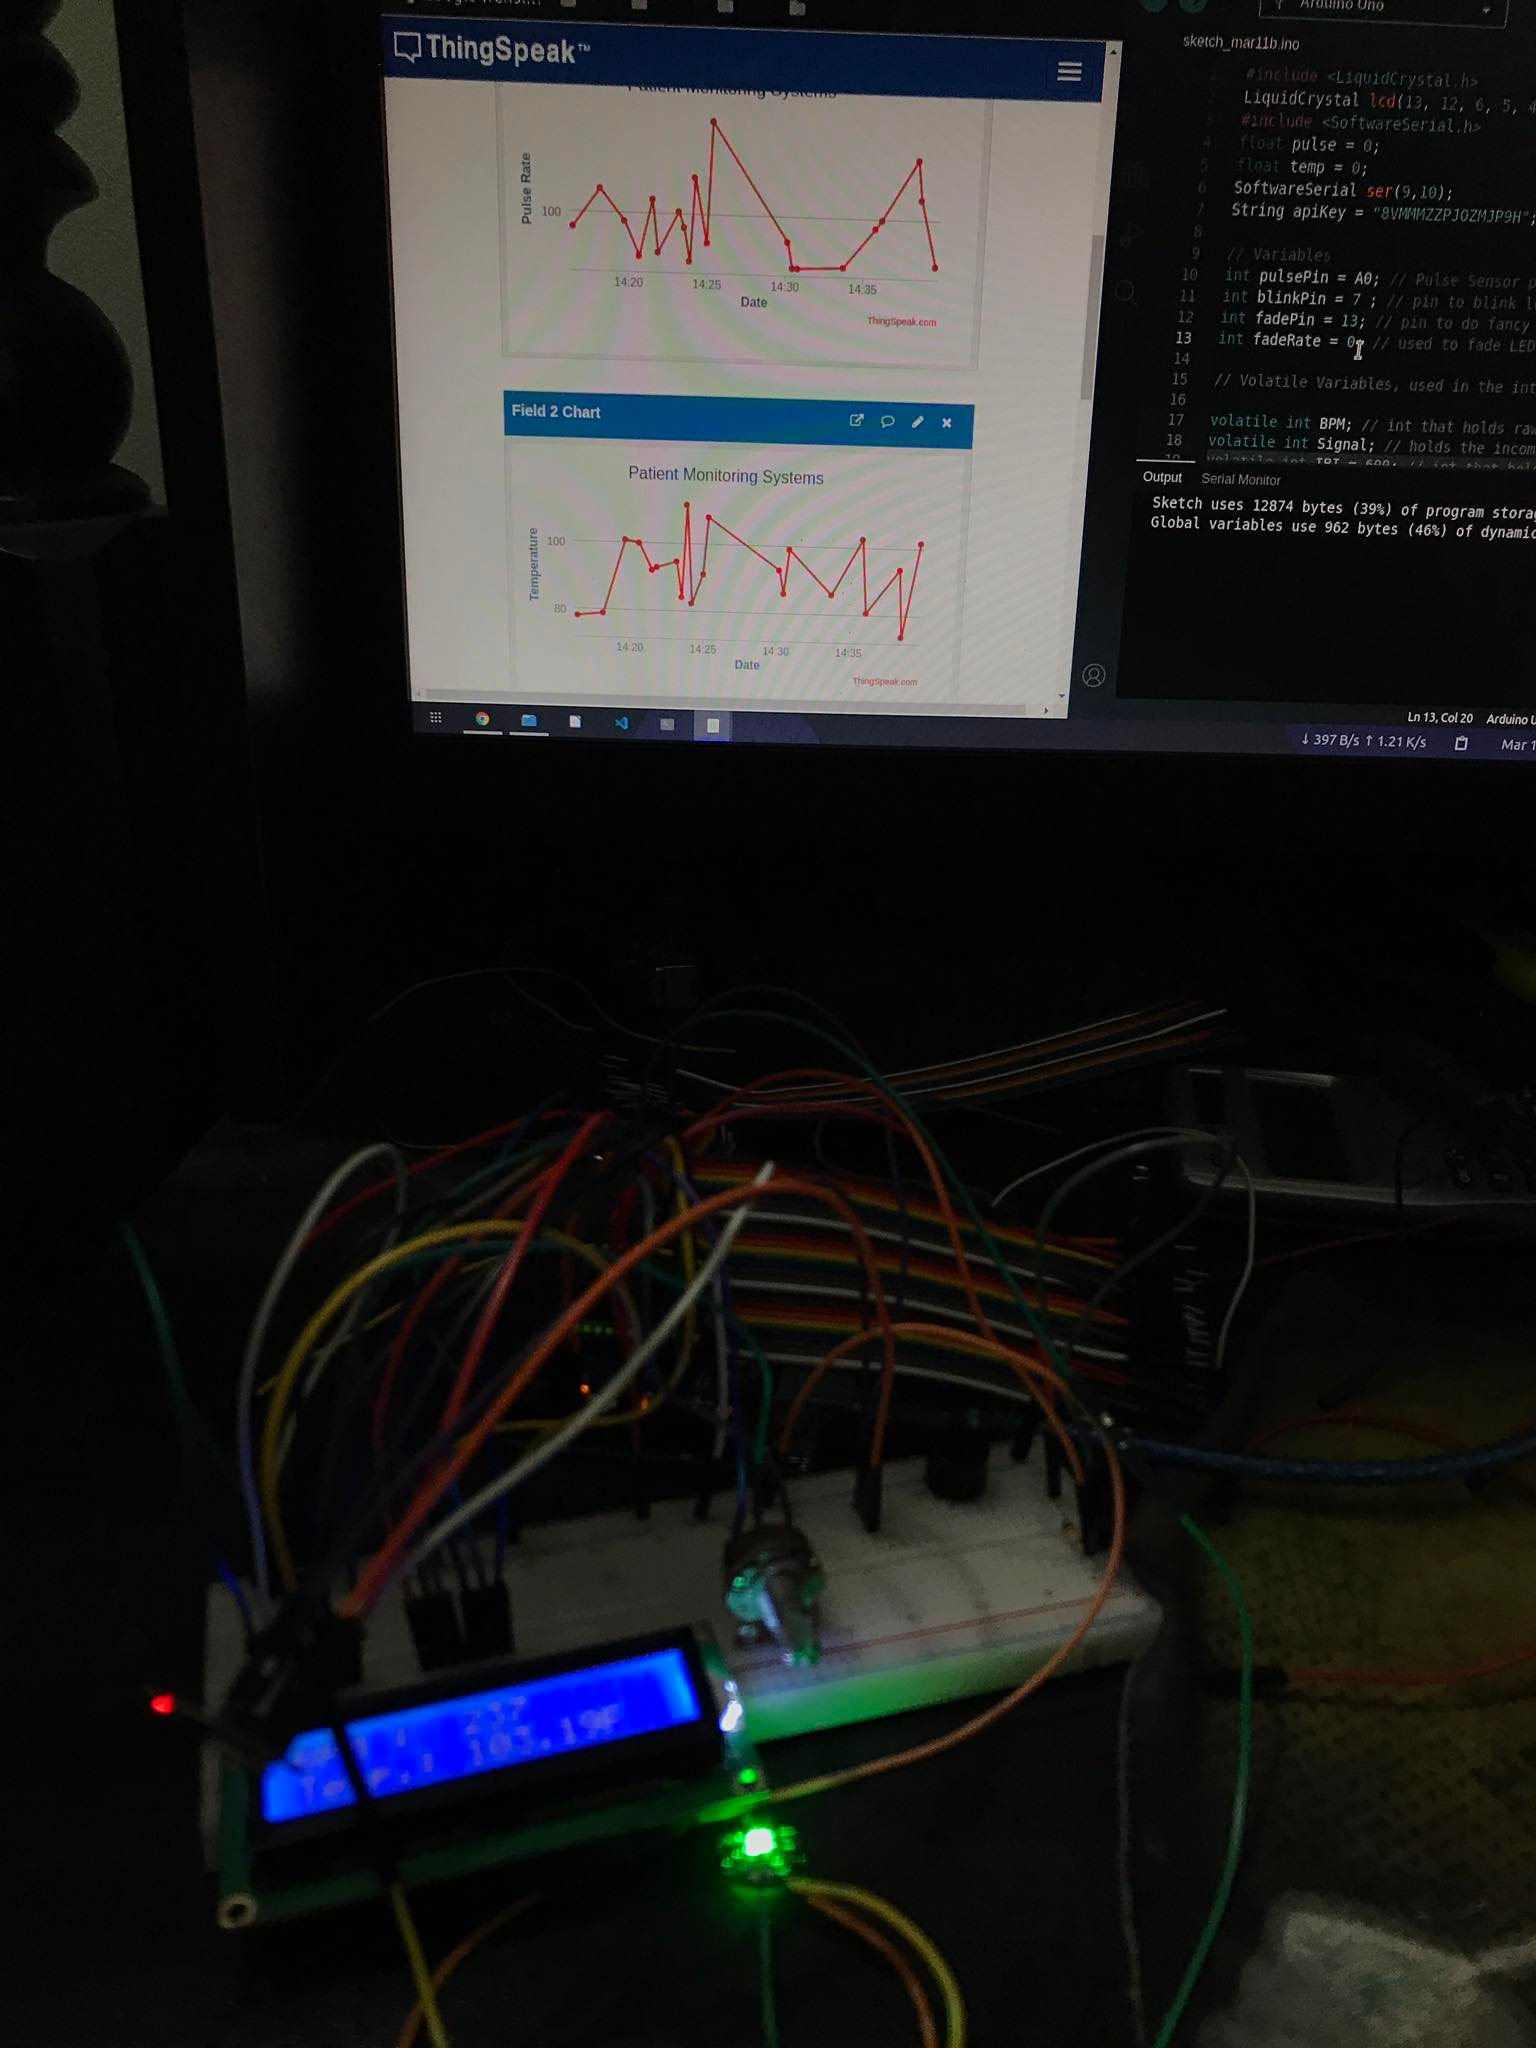
\includegraphics[width=0.25\textwidth]{fullProjectPic.jpg}
    \caption{Show data ThingSpeak }
    \label{fig:mesh1}
\end{figure}

\begin{figure}[h]
    \centering
    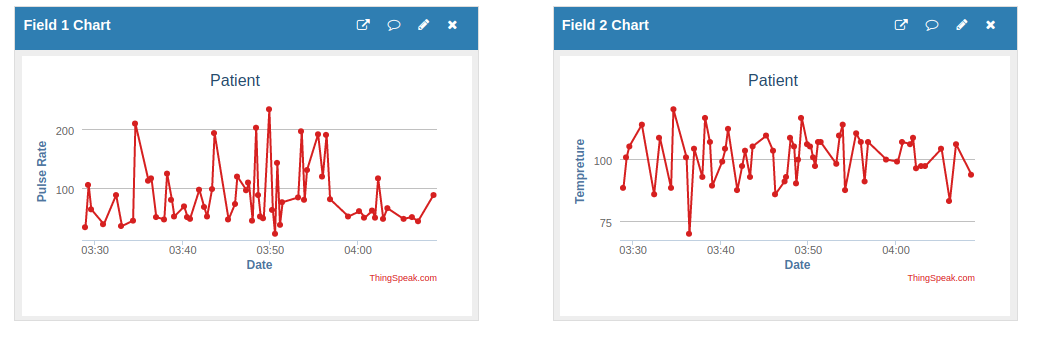
\includegraphics[width=.5\textwidth]{chart.png}
    \caption{Chart}
    \label{fig:mesh1}
\end{figure}

\section{Conclusion and Future Work}
The IoT-based health monitoring system for measuring blood pressure and the temperature has been successfully implemented. The system consists of hardware and software components, including sensors, microcontrollers, wireless communication modules, and a cloud-based platform for data storage and analysis. The system is capable of continuously monitoring the blood pressure and temperature of patients and transmitting the data to healthcare providers in real time. This allows for early detection of potential health issues and timely intervention, thereby improving patient outcomes and reducing healthcare costs. Future work could involve further refining the system to incorporate additional vital signs, such as heart rate and oxygen saturation, and incorporating machine learning algorithms to improve the accuracy of the readings and identify trends that may be indicative of underlying health issues. This could improve patient engagement and adherence to treatment plans. There are many exciting opportunities for further development of the IoT health monitoring system for blood pressure and temperature, and it has the potential to greatly improve patient outcomes and quality of life.
\section{Reference}
https://www.researchgate.net\\
http://repository.psa.edu.my\\
https://scholar.google.com\\
https://ieeexplore.ieee.org\\
https://pubmed.ncbi.nlm.nih.gov\\
https://aendt.com\\
https://www.ijert.org\\
https://iopscience.iop.org\\
https://www.pnrjournal.com\\
https://www.electronicsforu.com\\


\end{document}
